\subsubsection{Signaling Networks}
\begin{figure}[H]
\begin{multicols}{2}
\begin{figure}[H]
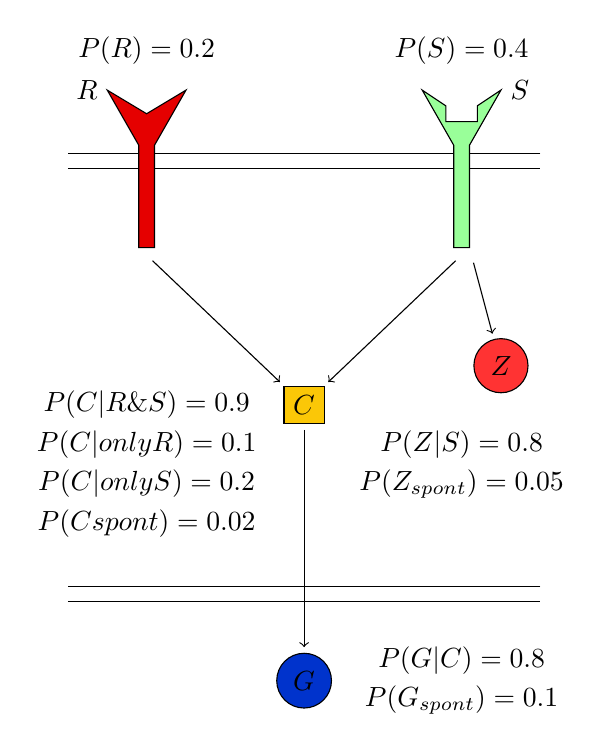
\begin{tikzpicture}
\draw (-3,0)--(3,0)(3,0.2)--(-3,0.2);
\draw[yshift=-5.5 cm] (-3,0)--(3,0)(3,0.2)--(-3,0.2);
\draw[fill=red!90!black,fill opacity=1] (-2.1,-1)node[name=re]{}--(-2.1,0.3)--(-2.5,1)node[left]{$R$}--(-2,0.7)--(-1.5,1)--(-1.9,0.3)--(-1.9,-1)--cycle;
\draw[fill=green!40!white,fill opacity=1] (2.1,-1)node[name=se]{}--(2.1,0.3)--(2.5,1)node[right]{$S$}--(2.2,0.8)--(2.2,0.6)--(1.8,0.6)--(1.8,0.8)--(1.5,1)--(1.9,0.3)--(1.9,-1)--cycle;
\node[draw,fill=yellow!80!red,shape=rectangle,name=c] at (0,-3){$C$};
\node at (-2,-3){$P(C|R\& S)=\num{0.9}$};
\node at (-2,-3.5){ $P(C|\text{ only } R)=\num{0.1}$};
\node at (-2,-4){$P(C|\text{ only }S)=\num{0.2}$};
\node at (-2,-4.5){$P(C \text{ spont})=\num{0.02}$};
\node at (2,-6.25){$P(G|C)=\num{0.8}$};
\node at (2,-6.75){$P(G_\text{spont})=\num{0.1}$};
\node at (2,1.5){$P(S)=\num{0.4}$};
\node at (-2,1.5){$P(R)=\num{0.2}$};
\node at (2,-3.5){$P(Z|S)=\num{0.8}$};
\node at (2,-4){$P(Z_\text{spont})=\num{0.05}$};
\node[draw,fill=red!80!white,shape=circle,name=z] at (2.5,-2.5){$Z$};
\node[draw,fill=blue!80!green,shape=circle,name=g] at (0,-6.5){$G$};
\draw[->,shorten <= 2pt, shorten >= 2pt] (re)--(c);
\draw[->,shorten <= 2pt, shorten >= 2pt] (se)--(c);
\draw[->,shorten <= 2pt, shorten >= 2pt] (se)--(z);
\draw[->,shorten <= 2pt, shorten >= 2pt] (c)--(g);
\end{tikzpicture}
\end{figure}
\columnbreak
\begin{align*}
P(G|C,R,S)&=P(R)P(S)P(C|R\& S)P(G|C)\\
&=\num{0.2}\cdot\num{0.4}\cdot\num{0.9}\cdot\num{0.8}=\num{0.0576}\\
P(G_{\text{spont}})&=0.1\\
P(Z_\text{signal})&=P(Z|S)P(S)=\num{0.4}\cdot\num{0.8}=\num{0.32}\\
P(G|C,R)&=\num{0.2}\cdot\num{0.1}\cdot\num{0.8}=\num{0.016}
\end{align*}
\end{multicols}
\end{figure}
Signaling networks consist of receptors that bind independently to \textbf{\underline{Ligands}}
\begin{itemize}[label={$\to$}]
\item the trigger same signal cascade of individually or collectively activated $\to $ genomic response.
\end{itemize}
Typically signaling is not deterministic, examples:
\begin{itemize}[label={$\to$}]
\item spontaneous trigger of the cascade with small probability
\item no signaling even if both/all receptors are active
\end{itemize}
Using statistical data we can for example establish the expression of a gene if the regular signaling cascade is activated.\\
Bayesion interference is mostly applied if the probability tables are not known a priori.
\begin{itemize}[label={$-$}]
\item A Bayesion network is constructed as a "directed acyclic graph" (DAG), i.e. the Graph has only directed edges and there is no probability to return to any of the nodes
\item parents of a node $X_i$: nodes $j$ that have an outgoing link to $x_i$; $\text{Par}_j(X_i)$
\item States of parents: "{}On" (1); "{}Off" (0) or other values $x_j$
\item configurations of a network witch n nodes
\begin{align*}
P(X_1=x_1,X_2=x_2,\ldots ,X_n=x_n)=\prod\limits_{i=1}^nP(X_i=x_i|\left\{\text{Par}_j(X_i)=X_j\right\})
\end{align*}
The r.h.s of the probability reflects that the probability of $x_i$ depends on the state of the parental sites (and not from any other). This decomposition is only possible if there are no loops in the graph.
\item In Bayesian inference the contditional probabilities are typically unknown. Instead we have usually a rough idea about the connectivity of a graph and a large data set of states.
\item General strategy:
\begin{itemize}[label={\labelitemiv}]
\item compose a graph with all known or hypothesized connections
\item define the direction of causality between nodes
\item assign the ranges of probabilities
\begin{itemize}[label={$\to$}]
\item run an optimization scheme $\to$ the outcome of the measurements serf as a reference for statistical tests.
\end{itemize}
\end{itemize}
\end{itemize}
\subsubsection{Static metabolic networks}
Metabolic networks are well suited for analysis since the networks represent the actual flow of material. Generically metabolic systems describe how one organic material is converted from one chemical to another (e.g. conversion of glucose to glucose-6-phosphate in the first reaction of glucolisis).\\
Compounds of interest in metabolic networks are represented as nodes, enzymatic reactions and transitions as edges.
\subsection{Stoichiometric networks}
\begin{figure}[H]
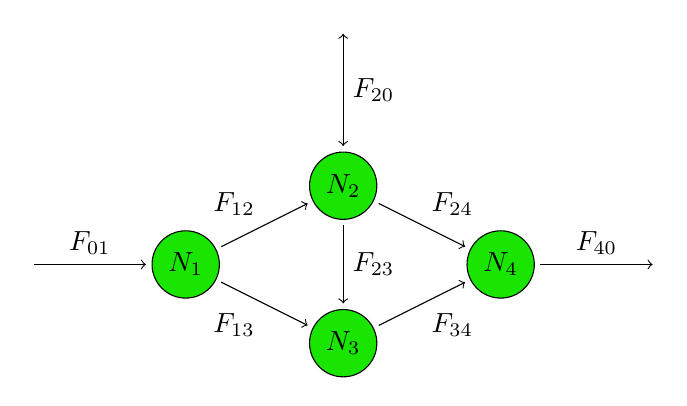
\begin{tikzpicture}
\node[draw,shape=circle,fill=green!90!red,name=n1] at (-2,0){$N_1$};
\node[draw,shape=circle,fill=green!90!red,name=n2] at (0,1){$N_2$};
\node[draw,shape=circle,fill=green!90!red,name=n3] at (0,-1){$N_3$};
\node[draw,shape=circle,fill=green!90!red,name=n4] at (2,0){$N_4$};
\draw[->, shorten <= 2pt, shorten >= 2pt] (-4,0)--(n1)node[midway,above]{$F_{01}$};
\draw[->, shorten <= 2pt, shorten >= 2pt] (n1)--(n2)node[midway,above left]{$F_{12}$};
\draw[->, shorten <= 2pt, shorten >= 2pt] (n1)--(n3)node[midway,below left]{$F_{13}$};
\draw[->, shorten <= 2pt, shorten >= 2pt] (n2)--(n3)node[midway,right]{$F_{23}$};
\draw[->, shorten <= 2pt, shorten >= 2pt] (n2)--(n4)node[midway,above right]{$F_{24}$};
\draw[->, shorten <= 2pt, shorten >= 2pt] (n3)--(n4)node[midway,below right]{$F_{34}$};
\draw[<->, shorten <= 2pt, shorten >= 2pt] (n2)--(0,3)node[midway,right]{$F_{20}$};
\draw[->, shorten <= 2pt, shorten >= 2pt] (n4)--(4,0)node[midway,above]{$F_{40}$};
\end{tikzpicture}
\end{figure}
We consider a stationary state, i.e. incoming and outgoing fluxes balance eacht other at a given node.\\
The constraint of conservation of mass leads to relations between fluxes, e.g. $F_{13}+F_{23}=F_{34}\quad (\ast)$. The set of relations is called stoichiometry.\\
\paragraph{Reminder} For bidirectional fluxes we consider two edges, e.g. $F_{20}$ and $F_{02}$.\\
It is easy to see that equations as $(\ast)$ are valid in the stationary state since the time evolution of $N_3$ is given by:
\begin{equation*}
\frac{dN_3(t)}{dt}=F_{13}(t)+F_{23}(t)-F_{34}(t)
\end{equation*}
